\documentclass[12pt,onecolumn]{article}
\usepackage[utf8]{inputenc}
\usepackage[spanish,es-noshorthands]{babel}
\usepackage{amsmath,amssymb}
\usepackage{graphicx}
\usepackage{xcolor}
\usepackage{tikz}
\usetikzlibrary{calc,arrows.meta}
\usepackage[legalpaper,top=2cm,bottom=2cm,left=2.2cm,right=2.2cm]{geometry}

% Colores por signo de carga
\definecolor{cargazul}{RGB}{40,40,210}   % positiva
\definecolor{cargarojo}{RGB}{210,40,40}  % negativa

\def\labelenumi{\arabic{enumi}.}
\def\theenumi{\arabic{enumi}}
\def\labelenumii{(\alph{enumii})}
\def\theenumii{\alph{enumii}}
\def\p@enumii{\theenumi.}
\pagestyle{plain}
\setcounter{secnumdepth}{0}

\begin{document}

\begin{center}

\includegraphics[height=1.8cm]{logo ubb.png}\\[0.3cm]
\textbf{F\'{\i}sica II (2026-2)}

\textbf{Tarea 1}\emph{: Fuerza y Campo el\'{e}ctrico de cargas puntuales y
distribuciones continuas}

\textit{Profesor: Arturo Fern\'{a}ndez P\'{e}rez}

\textbf{Plazo de Entrega: S\'{a}bado 29 de agosto a las 21:00 hrs.}
\end{center}

\bigskip

\begin{enumerate}
\item Tres cargas puntuales $q_{1}=-3$ $[nC]$, $q_{2}=2$ $[nC]$ y $q_{3}=5$
$[nC]$\ se ubican en un sistema de referencia, cuyas coordenadas y posiciones
(en cent\'{\i}metros, [cm]) se muestran en la Fig. 1. La carga $q_{1}$ se
encuentra a $12$ [cm] del origen. Determine:

\begin{itemize}
\item La fuerza el\'{e}ctrica neta $\vec{F}$ ejercida sobre la carga $q_{3}.$

\item El campo el\'{e}ctrico neto $\vec{E}$ en el punto (2,-8,3) [cm]
\end{itemize}

\begin{center}
\begin{tikzpicture}[scale=0.32, >=Stealth, line width=0.8pt]
    \draw[->,gray] (-11.8,0)--(11.8,0) node[right,font=\small]{$x$ [cm]};
    \draw[->,gray] (0,-8.8)--(0,6.4) node[above,font=\small]{$y$ [cm]};
    \node[gray,font=\scriptsize,above right] at (0.2,0.2){$O$};
    % q2 (+2nC) positiva -> azul
    \filldraw[cargazul] (-8,5) circle (5pt);
    \node[cargazul,above,font=\small] at (-8,5.7){$q_2$};
    \node[font=\scriptsize,left] at (-8.5,4.4){$(-8,5)$};
    % q3 (+5nC) positiva -> azul
    \filldraw[cargazul] (-10,-7) circle (5pt);
    \node[cargazul,below,font=\small] at (-10,-7.8){$q_3$};
    \node[font=\scriptsize,left] at (-10.5,-6.3){$(-10,-7)$};
    % q1 (-3nC) negativa -> rojo, a 12 cm y 30 grados bajo +x
    \filldraw[cargarojo] (10.39,-6) circle (5pt);
    \node[cargarojo,right,font=\small] at (10.9,-6){$q_1$};
    \draw[dashed,gray] (0,0)--(10.39,-6);
    \node[rotate=-30,font=\scriptsize] at (5.6,-2.7){$12$ cm};
    \draw (3.2,0) arc (0:-30:3.2);
    \node[font=\scriptsize] at (4.1,-1.1){$30^\circ$};
\end{tikzpicture}\\[-2pt]
{\small \textbf{Figura 1}}
\end{center}

\item Considere la siguiente configuraci\'{o}n de la Fig. 2, con
$q_{1}=q_{2}=3Q$ y $q_{3}=-4Q$. Si una part\'{\i}cula $q_{0}=-Q$ se ubica en
el punto P y considerando que $Q=10$ [$\mu C$] y $R=1,2$ [m],

\begin{itemize}
\item Dibuje las l\'{\i}neas de campo el\'{e}ctrico de las cargas $q_{1},$
$q_{2}$ y $q_{3}$ en el punto P.

\item Determine el campo el\'{e}ctrico neto $\vec{E}$ en el punto P,
inducido por $q_{1},$ $q_{2}$ y $q_{3}$

\item A partir del resultado anterior, determine la fuerza el\'{e}ctrica
neta $\vec{F}$ sobre la carga $q_{0}$
\end{itemize}

\begin{center}
\begin{tikzpicture}[scale=1.05, >=Stealth, line width=0.8pt]
    \draw[dashed,gray!70] (0,0) circle (2);
    \draw[->,gray] (-2.9,0)--(2.9,0) node[right,font=\small]{$x$};
    \draw[->,gray] (0,-2.9)--(0,2.9) node[above,font=\small]{$y$};
    \node[gray,font=\scriptsize,below left] at (0,0){$O$};
    % q1, q2 positivas (=3Q) -> azul ; q3 negativa (=-4Q) -> rojo
    \filldraw[cargazul] (90:2) circle (3.6pt);  \node[cargazul,above right,font=\small] at (90:2){$q_1$};
    \filldraw[cargazul] (0:2) circle (3.6pt);   \node[cargazul,above right,font=\small] at (0:2){$q_2$};
    \filldraw[cargarojo] (-50:2) circle (3.6pt); \node[cargarojo,below right,font=\small] at (-50:2){$q_3$};
    % punto P en (-R,0)
    \filldraw[black] (180:2) circle (3pt);   \node[above left,font=\small] at (180:2){$P$};
    % linea punteada q3 - origen (resalta el angulo y la posicion)
    \draw[dotted,line width=1pt] (0,0)--(-50:2);
    % radio R con etiqueta desplazada a la derecha
    \draw[->,gray] (0,0)--(58:2);
    \node[font=\small] at ($(58:1.25)+(0.32,0)$){$R$};
    % angulo 50 grados desde +x
    \draw (0:0.78) arc (0:-50:0.78);
    \node[font=\scriptsize] at (-25:1.08){$50^\circ$};
\end{tikzpicture}\\[-2pt]
{\small \textbf{Figura 2}}
\end{center}

\pagebreak

\item Una barra con densidad lineal de carga uniforme $\lambda =-8,5$ [$nC/m$]
se ubica sobre el eje $y$, como muestra la Fig. 3, entre $y=5$ [cm] e $y=18$
[cm]. Adem\'{a}s, en el punto $P$, de coordenadas (5,-7) [cm] se ubica una
carga puntual $q=16$ [$nC$]. Determine:

\begin{itemize}
\item El campo el\'{e}ctrico $\vec{E}$ inducido por la barra en el punto $P$

\item La fuerza el\'{e}ctrica $\vec{F}$ sobre la carga $q.$
\end{itemize}

\begin{center}
\begin{tikzpicture}[scale=0.22, >=Stealth, line width=0.8pt]
    \draw[->,gray] (-3,0)--(8,0) node[right,font=\small]{$x$ [cm]};
    \draw[->,gray] (0,-9.5)--(0,20.5) node[above,font=\small]{$y$ [cm]};
    \node[gray,font=\scriptsize,below left] at (0,0){$O$};
    % barra (lambda<0) roja sobre el eje y, de y=5 a y=18
    \draw[cargarojo,line width=3pt] (0,5)--(0,18);
    \node[cargarojo,right,font=\small] at (0.6,11.5){$\lambda$};
    \draw[gray] (-0.5,5)--(0.5,5);   \node[font=\scriptsize,left] at (-0.7,5){$y{=}5$};
    \draw[gray] (-0.5,18)--(0.5,18); \node[font=\scriptsize,left] at (-0.7,18){$y{=}18$};
    % carga puntual q (positiva) azul en P=(5,-7)
    \draw[dashed,gray] (0,-7)--(5,-7); \draw[dashed,gray] (5,0)--(5,-7);
    \filldraw[cargazul] (5,-7) circle (5pt);
    \node[cargazul,right,font=\small] at (5.7,-7){$q$};
    \node[font=\scriptsize,below] at (5,-8.4){$P(5,-7)$};
\end{tikzpicture}\\[-2pt]
{\small \textbf{Figura 3}}
\end{center}

\item Considere un \emph{segmento de circunferencia} de radio $R=15,0$ [cm]
que se ubica entre los \'{a}ngulos $\phi_{1}=\frac{5\pi}{6}$ y
$\phi_{2}=\frac{4\pi}{3}$ (medidos desde el eje $x^{+}$), como muestra la
Fig. 4. Si \'{e}ste posee una densidad de carga lineal uniforme
$\lambda =4,0$ [$\mu C/m$],

\begin{itemize}
\item Determine el campo el\'{e}ctrico $\vec{E}$ en un punto P en el eje del segmento circular,
a una distancia $z_{0}=8,0$ [cm] de su centro.

\item Si en ese punto se ubica una carga puntual $q=7,0$ [$\mu C$] determine la fuerza el\'{e}ctrica $\vec{F}$ ejercida sobre ella.
\end{itemize}

\begin{center}
\begin{tikzpicture}[scale=1.05, >=Stealth, line width=0.8pt,
    x={(-0.52cm,-0.36cm)}, y={(1cm,0cm)}, z={(0cm,1cm)}]
    % ejes (angulos medidos desde +x)
    \draw[->,gray] (0,0,0)--(2.5,0,0) node[below,font=\small]{$x$};
    \draw[->,gray] (0,0,0)--(0,2.5,0) node[right,font=\small]{$y$};
    \draw[->,gray] (0,0,0)--(0,0,2.7) node[above,font=\small]{$z$};
    % segmento de circunferencia (lambda>0) azul, phi de 150 a 240 (5pi/6 a 4pi/3)
    \draw[cargazul,line width=1.9pt]
        plot[domain=150:240,samples=50,variable=\t] ({1.6*cos(\t)},{1.6*sin(\t)},0);
    \node[cargazul,font=\small] at ({1.98*cos(196)},{1.98*sin(196)},0.12){$\lambda$};
    % radios a los extremos del arco, con los angulos phi1 y phi2 (desde +x)
    \draw[dashed,gray] (0,0,0)--({1.6*cos(150)},{1.6*sin(150)},0);
    \node[font=\scriptsize] at ({1.85*cos(150)},{1.85*sin(150)},0.12){$\phi_1$};
    \draw[dashed,gray] (0,0,0)--({1.6*cos(240)},{1.6*sin(240)},0);
    \node[font=\scriptsize] at ({1.82*cos(240)},{1.82*sin(240)},0.12){$\phi_2$};
    \node[font=\scriptsize] at ({0.9*cos(150)},{0.9*sin(150)},0.22){$R$};
    % punto P sobre el eje z, a distancia z0 del centro
    \draw[dashed,gray] (0,0,0)--(0,0,1.8);
    \filldraw[black] (0,0,1.8) circle (1.8pt);
    \node[right,font=\small] at (0,0.08,1.8){$P$};
    \node[font=\scriptsize,left] at (0,-0.05,1.0){$z_0$};
\end{tikzpicture}\\[-2pt]
{\small \textbf{Figura 4}}
\end{center}

\item Se tiene un sistema formado por dos l\'{\i}neas cargadas uniformemente, ubicadas como se muestra en la Fig. 5. La l\'{\i}nea 1 tiene densidad de carga $\lambda_{1}=-18$ $[\mu C/m]$. La l\'{\i}nea 2 tiene carga total $Q_{2}=70$ $[\mu C]$. Considerando que $R=20$ [cm], determine:

\begin{itemize}
\item La densidad de carga de la l\'{\i}nea 2 ($\lambda_{2}$) y la carga total de la l\'{\i}nea 1 ($Q_{1}$).

\item El campo el\'{e}ctrico $\vec{E}_{1}$ que genera la l\'{\i}nea 1 en el origen del sistema de coordenadas.

\item El campo el\'{e}ctrico $\vec{E}_{2}$ que genera la l\'{\i}nea 2 en el origen del sistema de coordenadas.

\item El campo el\'{e}ctrico neto $\vec{E}_{T}$ en el origen del sistema de coordenadas.
\end{itemize}

\begin{center}
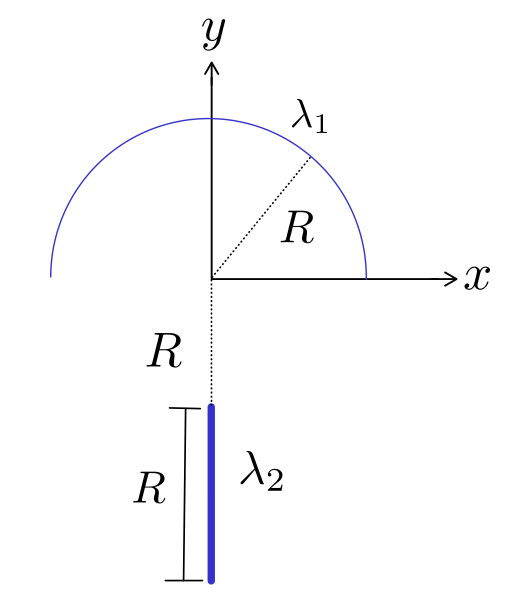
\includegraphics[width=6.5cm]{Electro1.png}\\[-1pt]
{\small \textbf{Figura 5}}
\end{center}

\end{enumerate}

\end{document}
